\chapter{SRAM22}

SRAM22 is an open-source SRAM generator for the Skywater 130nm open-source process.
SRAM22 programatically generates SRAM blocks by consuming:
+ A TOML configuration file, such as the one shown below.
+ A set of hard macros, including standard cells, a sense amplifier, and SRAM bitcells.
+ A summary of process design rules.
+ A Substrate PDK, which provides a parametric transistor generator.

SRAM22 does not attempt to be process-portable, even though many of the above components
can, in principle, be swapped out to port SRAM22 to a new process.

An example TOML configuration file is shown below:

\begin{minted}{toml}
num_words = 32
data_width = 32
mux_ratio = 2
write_size = 32
control = "ReplicaV1"
pex_level = "rcc"
\end{minted}

These options configure the width/depth of the SRAM, the column muxing ratio, and the write mask granularity.
Since running PEX can often take hours or even days, the \verb|pex_level| option allows users to specify
the level of accuracy desired.

An invocation of SRAM22 produces all collateral required for integrating SRAM into a digital flow, including:
\begin{itemize}
\item A SPICE netlist.
\item A GDS layout.
\item A LEF file, identifying pin and blockage locations.
\item A Liberty file, specifying timing constraints.
\item A Verilog behavioral model.
\end{itemize}

Users can also request that SRAM22 run checks on the generated SRAM block, including:
\begin{itemize}
\item Running LVS.
\item Running DRC.
\item Running a sanity-check transistor-level functional simulation.
\end{itemize}

The complete source code for SRAM22 is available on \href{https://github.com/rahulk29/sram22}{GitHub}.

\ref{sec:sram-architecture} describes the architecture of the generated SRAM blocks.
\ref{sec:sram-layout-generation} describes how SRAM22 programatically generates layout.

\section{Architecture} \label{sec:sram-architecture}

SRAM22 generates self-timed SRAMs. Figure \ref{fig:sram22-block-diagram} shows a block diagram
of the macros generated by SRAM22.

\begin{figure}[H] \centering
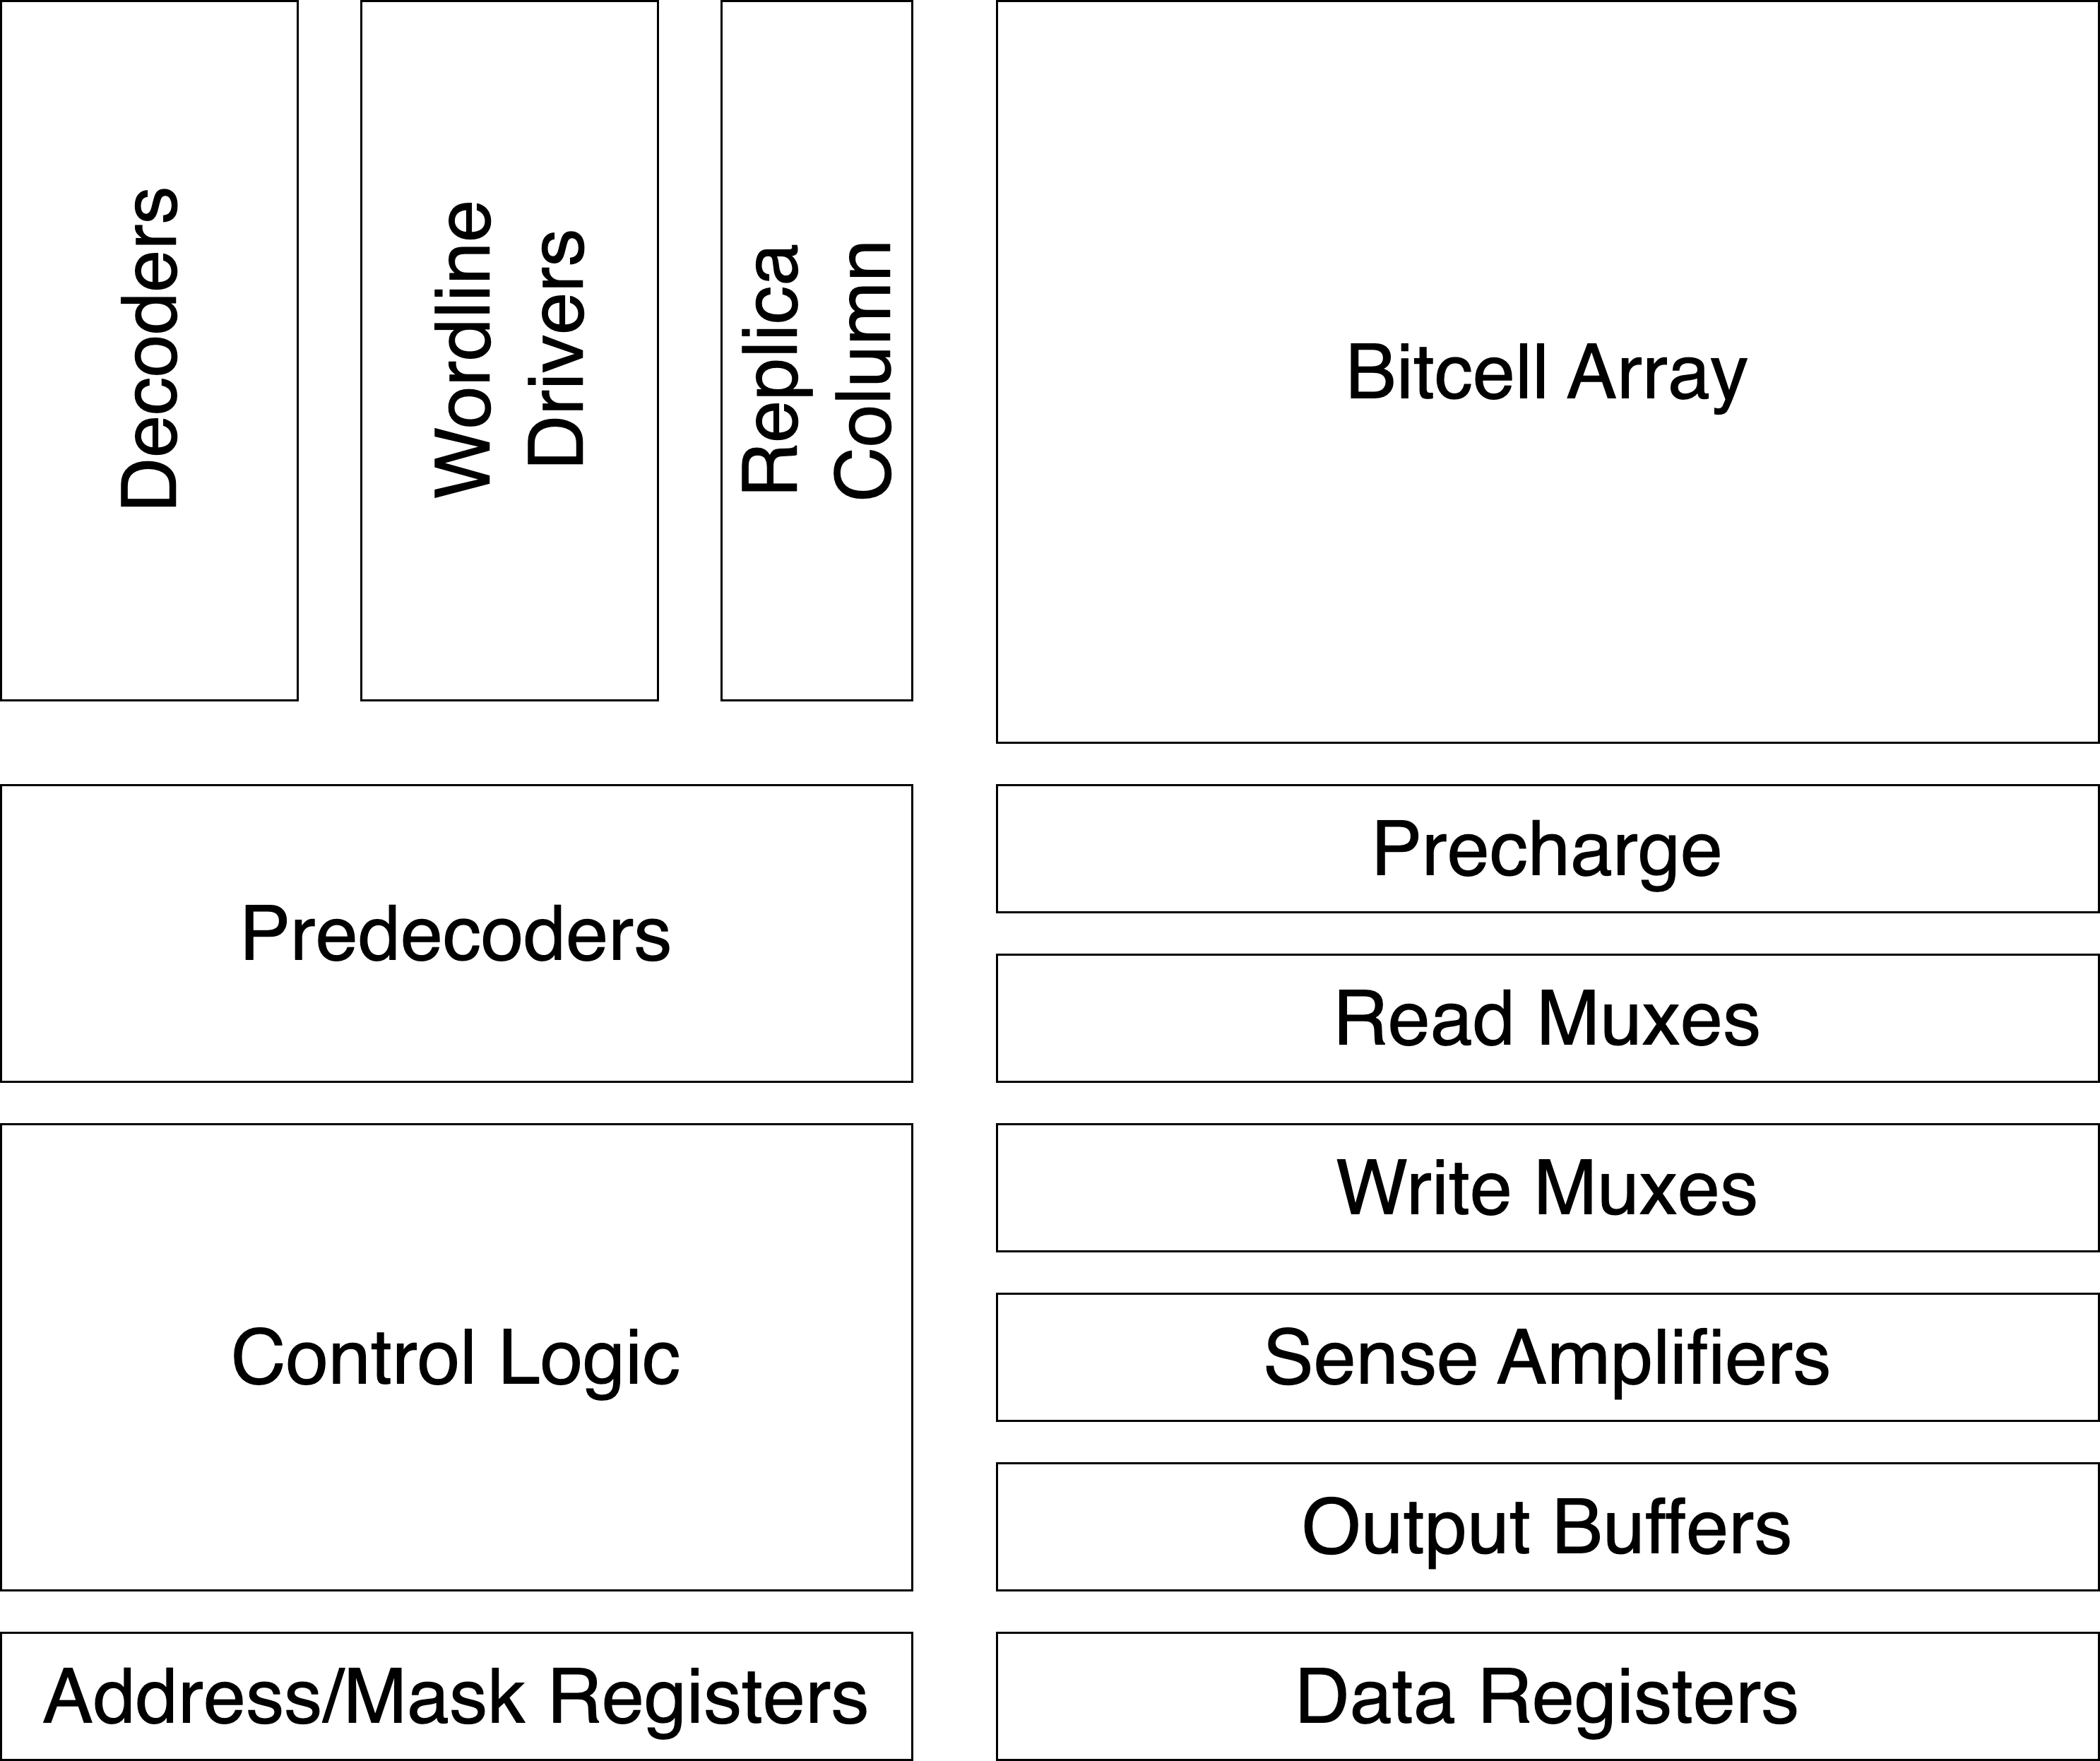
\includegraphics[width=0.8\textwidth]{figures/sram22_block_diagram.png}
\caption{A block diagram of an SRAM macro generated by SRAM22. \label{fig:sram22-block-diagram}}
\end{figure}

The internally generated sense amplifier clock is derived
from a replica bitline. Details on the design of the replica timing mechanism can be found in \ref{sec:replica-bitline}.

\subsection{Replica Bitline} \label{sec:replica-bitline}

The purpose of the replica bitline is to accurately track the discharge delay of the true bitlines across
process, voltage, and temperature variations. Since SRAM cells are composed of special transistors
not ordinarily used in logic cells, timing mechanisms based on logic (such as inverter chains) do not
track the true bitlines well.

To minimize power consumption due to charging and discharging the bitlines,
the replica delay can be designed to fire the sense amplifiers when just enough voltage difference
has accumulated. This minimum voltage depends primarily on the sensitivity and offset voltage of the
sense amplifiers.

We present a replica bitline design based on \cite{replicabl}.
We use a design in which there are $N$ replica columns, each of which is smaller than a regular column by a factor of $K$. In other words, if a regular SRAM column has $h$ cells, each replica column will have $h/K$ cells.
The $N$ replica columns are connected in parallel to reduce timing variation due to random effects in active replica cells.
An inverter senses the discharging replica bitline and fires sense amplifiers.

We now present a method for selecting the values of $N$ and $K$.

We assume that the following values are known (eg. extracted from simulation) and constant:
\begin{itemize}
\item The bitline capacitance $C_{bl}$
\item The nominal SRAM cell on current, $I_{cell,0}$
\item The standard deviation of SRAM cell current, $\sigma_{I_{cell}}$
\item The standard deviation of the sense amplifier offset voltage $V_{os}$
\item The threshold $V_{flip}$ at which an inverter output flips from low to high
\item The supply voltage $V_{DD}$
\end{itemize}

A read error occurs if the sense amps fire before sufficient voltage difference develops on the true bitlines.

For this analysis, we suppose that we must tolerate up to $M_1$ standard deviations of sense amp offset voltage
and $M_2$ standard deviations of SRAM cell current.

The total bitline capacitance of the replica columns is $ C_{replica} = N/K C_{bl}. $
If this capacitance is discharged by a current $I_{replica}$, the time at which the sense amps are enabled is
\begin{equation}
T_{SAE} = \frac{C_{replica}}{I_{replica}}\left( V_{DD} - V_{flip} \right).
\end{equation}
Note that nominally $I_{replica} = N I_{cell}$, since the replica column contains $N$ replica cells in parallel.

For a correct read, the voltage difference at the input of the sense amps must be larger than $M_1 V_{os}.$
If the true bitlines are discharged by a current $I_{cell}$, we must have
\begin{equation}
T_{SAE} > \frac{C_{bl}}{I_{cell}} M_1 V_{os}.
\end{equation}

The worst case conditions occur when:
\begin{enumerate}
\item The cell being read is slow: $ I_{cell} = I_{cell,0} - M_2 \sigma_{I_{cell}}. $

\item The replica cells are fast: $ I_{replica} = N I_{cell} + M_2 \sqrt{N} \sigma_{I_{cell}}. $

\item The sense amplifiers have the maximal offset voltage $M_1 V_{os}$.
\end{enumerate}

We now derive a condition for correctness under the worst case conditions.

The worst case (earliest) time at which the sense amps are fired is

\begin{equation} \label{eq:tsae-max}
T_{SAE} = \frac{C_{replica}}{I_{replica}} \left( V_{DD} - V_{flip} \right)
= \frac{ N C_{bl}  \left(V_{DD} - V_{flip} \right) }{ K \left( N I_{cell,0} + M_2 \sqrt{N} \sigma_{I_{cell}} \right)}.
\end{equation}

The worst case (latest) time at which sufficient bitline voltage margin has accumulated is

\begin{equation} \label{eq:tmin}
T_{min} = \frac{M_1 C_{bl} V_{os}}{I_{cell} - M_2 \sigma_{I_{cell}}}.
\end{equation}

For correct operation, \ref{eq:tsae-max} must be larger than \ref{eq:tmin}. Thus, the correctness constraint is

\begin{equation} \label{eq:sae-correctness}
\frac{C_{bl}  \left( V_{DD} - V_{flip}\right)}{K \left( I_{cell,0} + M_2 \frac{1}{\sqrt{N}} \sigma_{I_{cell}} \right)} >
\frac{M_1 C_{bl} V_{os}}{I_{cell} - M_2 \sigma_{I_{cell}}}.
\end{equation}

\ref{eq:sae-correctness} shows that increasing $N$ mitigates the variance of the replica cells,
though it does nothing to alleviate the variance of the SRAM cells.

A simple heuristic to select $N$ and $K$ is to solve for $K$ based on the nominal cell current and worst case
sense amp offset voltage:

\begin{align} \label{eq:k-heuristic}
\frac{C_{bl} \left( V_{DD} - V_{flip} \right) }{K I_{cell,0}}
&= \frac{C_{bl} M_1 V_{os}}{I_{cell,0}} \\
\implies K &= \frac{V_{DD} - V_{flip}}{M V_{os}}
\end{align}

The value of $N$ is then determined by finding the minimumm value of $N$ that satisfies \ref{eq:sae-correctness}.
Since $N$ does nothing for the SRAM cell current variation, this approach may not always yield a positive solution for $N$.
Such cases can be solved iteratively by decreasing $K$ and then searching for an $N$ satisfying \ref{eq:sae-correctness}.


\section{Layout Generation} \label{sec:sram-layout-generation}

SRAM22 exercises many of the layout APIs described in \ref{sec:layout-entry}.
This section describes a few representative examples.

This section is organized as follows:
\begin{enumerate}
\item \ref{sec:bitcell-array-layout} describes how Substrate tiling APIs are used to produce SRAM bitcell arrays from foundry-provided cells.
\item \ref{sec:precharge-layout} describes how Substrate's raw layout APIs can be used to produce very compact layouts.
\item \ref{sec:control-logic-layout} describes how Substrate's routing APIs handle custom digital logic, where layout area is dominated
  by standard cell area, rather than by routing performance, and productivity is important.
\end{enumerate}


\subsection{Bitcell Array} \label{sec:bitcell-array-layout}

SRAM22 uses many of the tiling APIs described in \ref{sec:placement-utilities}.
As an example, consider the (toy) 8x8 bitcell array shown in \ref{fig:bitcell8x8}.

\begin{figure}[H] \centering
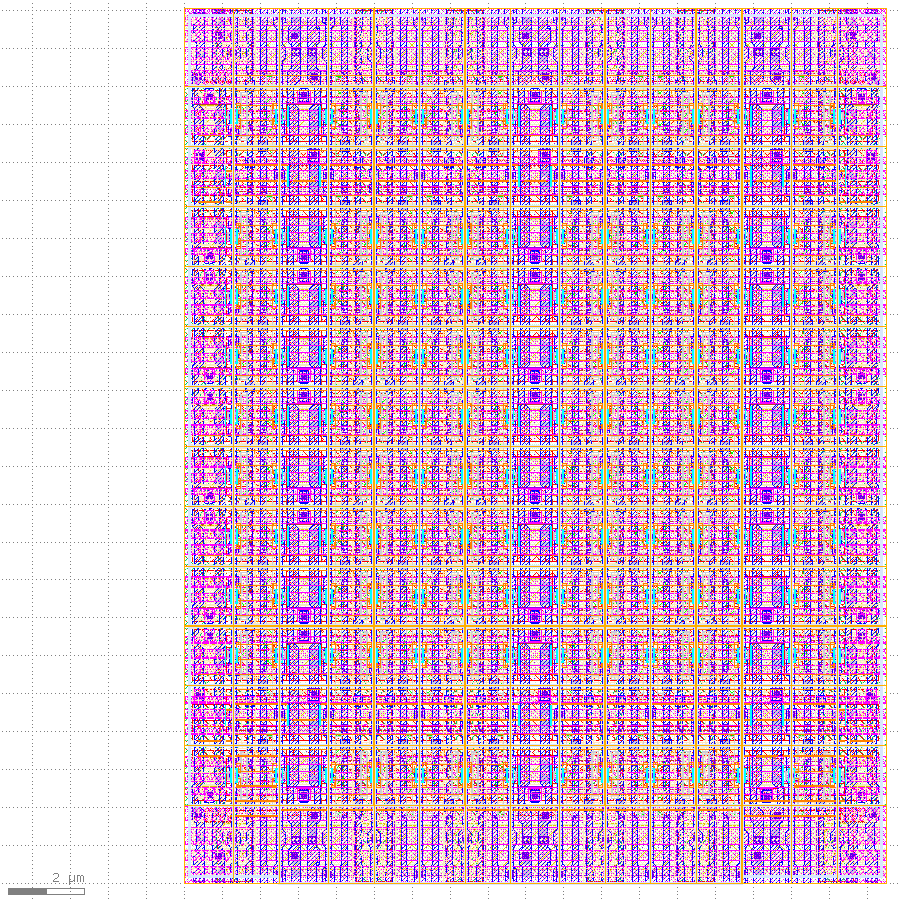
\includegraphics[width=0.8\textwidth]{figures/bitcell8x8.png}
\caption{An 8x8 SRAM bitcell array tiled using Substrate. \label{fig:bitcell8x8}}
\end{figure}

The bitcell array has several structural features commonly found in SRAM bitcell arrays:
\begin{itemize}
\item One horizontal tap row for every 8 rows of cells.
\item One vertical tap column for every 4 columns of cells. Note that this array was
  generated for a column mux ratio of 4. For a column mux ratio of 8, the tap columns
  would be placed every 8 cells.
\item Special row end, column end, and corner cells.
\item Each SRAM bitcell shares bitline and power contacts with its neighbors.
  As a result, each cell in a row is reflected horizontally with respect to the cell preceeding it.
  Similarly, each cell in a column is reflected vertically with respect to the cell above it.
\end{itemize}

The requirements for special edge and corner cells makes this a natural fit for a ninepatch tiler.
To use the ninepatch tiling API, we must first partition the bitcell into the nine ninepatch regions (center, four edges, and four corners).

The center cell is the unit that tiles in both the horizontal and vertical dimensions. For the example shown above,
the center cell contains a horizontal tap row, 8 rows of 4 bitcells, and a vertical tap column. Tiling this cell
will produce an array with the desired frequency of taps (one horizontal tap every 8 rows, and one vertical tap every 4 columns).
An image of the center cell is shown in \ref{fig:bitcell-center}. Note that we have placed taps at the top and left edges of the cell.
We account for this when designing the edge and corner cells.

\begin{figure}[H] \centering
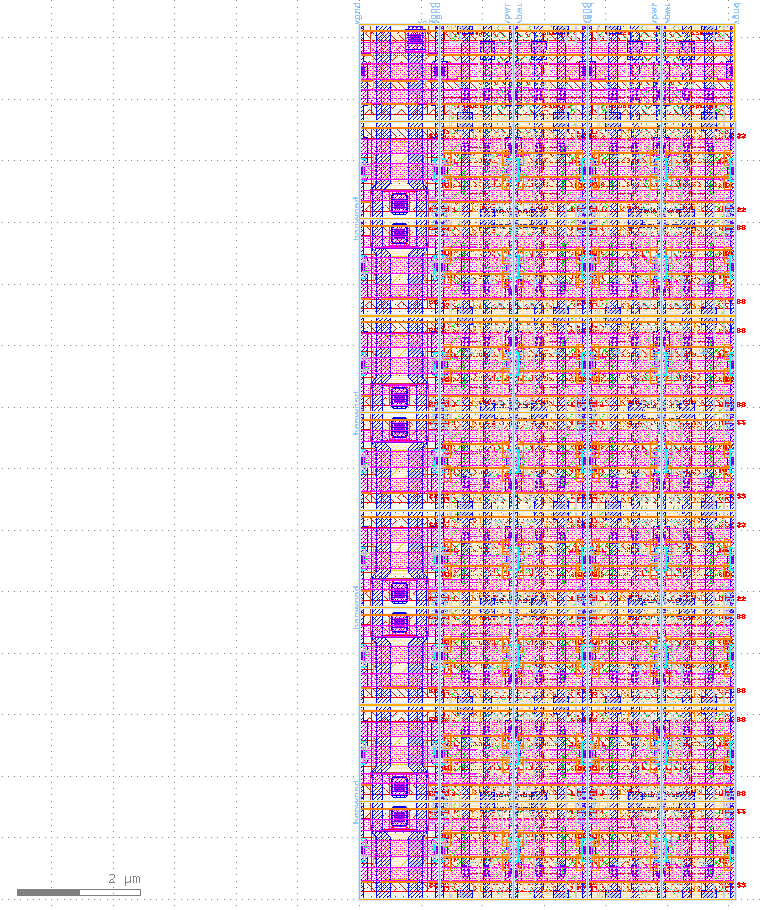
\includegraphics[width=0.5\textwidth]{figures/bitcell_center.png}
\caption{The center ninepatch cell for the bitcell array shown in \ref{fig:bitcell8x8}. \label{fig:bitcell-center}}
\end{figure}

The remainder of the ninepatch tiles are shown in \ref{fig:bitcell-ninepatch-tiles}.
Since the center cell contains taps at the left and top edges, the left/top ninepatch cells
do not contain internal tap structures, whereas the right/bottom cells do.
\begin{figure}[H] \centering
\begin{subfigure}[b]{0.22\textwidth} \centering
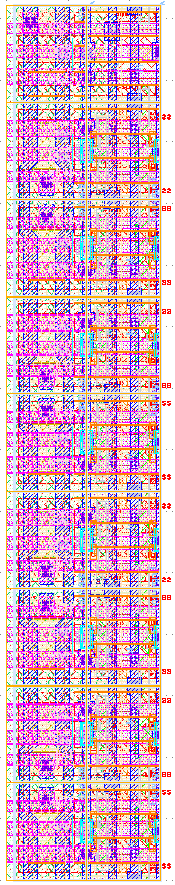
\includegraphics[width=\textwidth]{figures/bitcell_left.png}
\caption{Left edge}
\end{subfigure}
\hfill
\begin{subfigure}[b]{0.22\textwidth} \centering
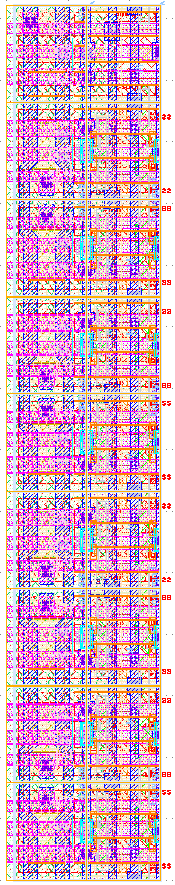
\includegraphics[width=\textwidth]{figures/bitcell_left.png}
\caption{Left edge}
\end{subfigure}
\hfill
\begin{subfigure}[b]{0.22\textwidth} \centering
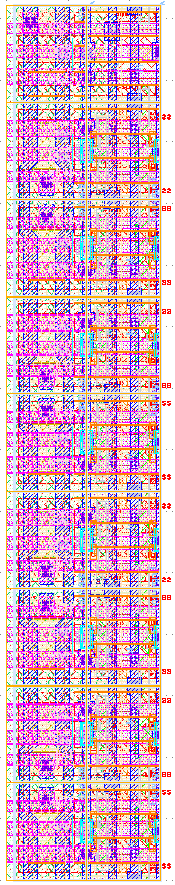
\includegraphics[width=\textwidth]{figures/bitcell_left.png}
\caption{Left edge}
\end{subfigure}
\hfill
\begin{subfigure}[b]{0.22\textwidth} \centering
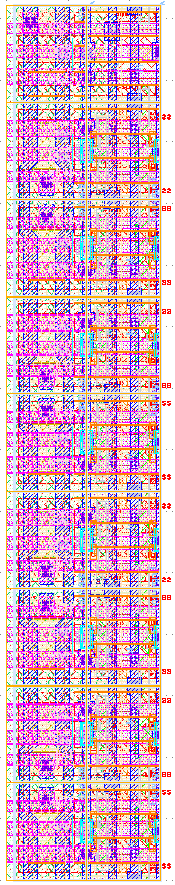
\includegraphics[width=\textwidth]{figures/bitcell_left.png}
\caption{Left edge}
\end{subfigure}

\caption{The off-center ninepatch cells for the bitcell array shown in \ref{fig:bitcell8x8}. \label{fig:bitcell-ninepatch-tiles}}
\end{figure}

% #figure(
%   table(
%     columns: 4,
%     align: center,
%     image("figures/bitcell_left.png", width: 22%),
%     image("figures/bitcell_right.png", width: 22%),
%     image("figures/bitcell_top.png", width: 22%),
%     image("figures/bitcell_bot.png", width: 22%),
%     image("figures/bitcell_ul.png", width: 22%),
%     image("figures/bitcell_ll.png", width: 22%),
%     image("figures/bitcell_ur.png", width: 22%),
%     image("figures/bitcell_lr.png", width: 22%),
%   ),
%   caption: [
%     The off-center ninepatch cells for the bitcell array shown in @bitcell8x8.
%     Top row (from left to right): left edge, right edge, top edge, bottom edge.
%     Bottom row (from left to right): upper left corner, lower left corner, upper right corner, lower right corner.
%   ],
% ) <bitcell-ninepatch-tiles>

Once we have generated layouts of the ninepatch cells, tiling them 
using Substrate's \verb|NpTiler| is fairly straightforward:

\begin{minted}{rust}
let tiler = NpTiler::builder()
    .set(Region::CornerUl, &corner_ul)
    .set(Region::Left, &left)
    .set(Region::CornerLl, &corner_ll)
    .set(Region::Top, &top)
    .set(Region::Center, &center)
    .set(Region::Bottom, &bot)
    .set(Region::CornerUr, &corner_ur)
    .set(Region::Right, &right)
    .set(Region::CornerLr, &corner_lr)
    .nx(nx)
    .ny(ny)
    .build();
\end{minted}

Each of the nine ninepatch region tiles are composite cells; they each contain
multiple foundry-provided primitive cells. To generate these tiles, we use Substrate's \verb|GridTiler|.

For example, \ref{fig:bitcell-left-cell-code} shows a portion of the code for generating the left edge cell.
\begin{figure}[H] \centering
\begin{minted}{rust} 
let cell_row: Vec<OptionTile> = into_vec![rowend_replica, cell];
let cell_opt1a_row: Vec<OptionTile> = into_vec![rowenda_replica, cell_opt1a];
let hstrap: Vec<OptionTile> = into_vec![rowend_hstrap, hstrap];

let mut grid = Grid::new(0, 0);
grid.push_row(hstrap);
for _ in 0..self.params.hstrap_ratio / 2 {
    grid.push_row(cell_opt1a_row.clone());
    grid.push_row(cell_row.clone());
}

let mut grid_tiler = GridTiler::new(grid);
\end{minted}
\caption{A code snippet for generating the left edge cell of an SRAM bitcell array. \label{fig:bitcell-left-cell-code}}
\end{figure}

This code:
\begin{enumerate}
\item Creates three rows of 2 cells each: one normal bitcell row, one bitcell row with slight modifications
  to geometry for OPC, and one row for taps. These rows are just collections of cells; they are not
  yet placed in the actual cell layout.
\item Adds the tap row as the first (topmost) row in the grid. This row will align with the topmost row
  of the ninepatch center cell (\ref{fig:bitcell-center}), which is also a tap row.
\item Adds alternating rows of regular bitcells and modified-OPC bitcells. Eight rows are added in total,
  since \verb|self.params.hstrap_ratio| is 8 here. As is evident from the code, the frequency of horizontal
  tap rows can easily be adjusted.
\item Creates a \verb|GridTiler| instance to place all of the cells.
\end{enumerate}

The lowest level of cells in the hierarchy (eg. \verb|cell|, \verb|cell_opt1a| in the code above) are imported
into Substrate using hard macros (\ref{sec:hard-macros}).

In addition to tiling geometry, we also expose relevant ports from each of the tilers. This allows
other generators to figure out how to connect to the bitcell array. For example, we expose ports for
each of the wordlines, bitlines, and power strap connections. The code to do this is omitted for brevity,
but can be found in the SRAM22 source code.

Although bitcell tiling is not fundamentally a hard problem, we believe that the approach of decomposing
the problem into reasonably intuitive parts (such as grid and ninepatch tiling) is better and more easily understood
than the alternative, ``simpler'' method of writing a double for loop
with edge cases to handle the array edge cells and periodic taps.

\subsection{Precharge} \label{sec:precharge-layout}

The precharge cell illustrates how to use Substrate to produce compact, tileable layouts.
The SRAM bitcell width in the Skywater 130nm process is \SI{1.2}{\micro\meter}.
The minimum metal 1 line and space is \SI{0.28}{\micro\meter},
meaning that at most 4 M1 tracks will fit within the bitcell pitch. However, since minimum-sized vias are wider
than the minimum M1 width, we are practically limited to around 3 M1 tracks. There are four signals involved
in the precharge circuit: the bitline, complementary bitline, VDD, and active low precharge enable.
Thus, routing performance is critical.

The final precharge cell is shown in \ref{fig:precharge-final}.

\begin{figure}[H] \centering
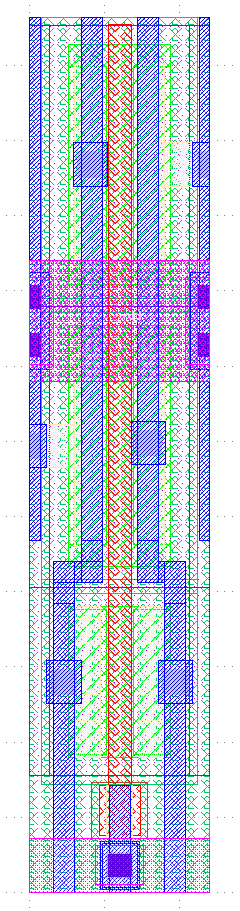
\includegraphics[angle=90, width=\textwidth]{figures/precharge_final.png}
\caption{The pitch-matched precharge cell in SRAM22. \label{fig:precharge-final}}
\end{figure}

Before we describe how SRAM22 generates this layout, we first highlight some important features:
\begin{itemize}
\item VDD is routed into the cell from metal 2 (pink) and drops onto split tracks on metal 1 (blue).
  The split tracks of adjacent cells abut to form a full track.
\item The bitlines jog slightly to make space to enable routing precharge enable to the gates of the precharge devices.
\item The total capacitance (and therefore total wire length) on the bitline and bitline complement nets must be approximately equal.
\end{itemize}

To generate the precharge cell layout, we start by instantiating the three precharge transistors, as shown in \ref{fig:precharge-transistors}.

\begin{figure}[H] \centering
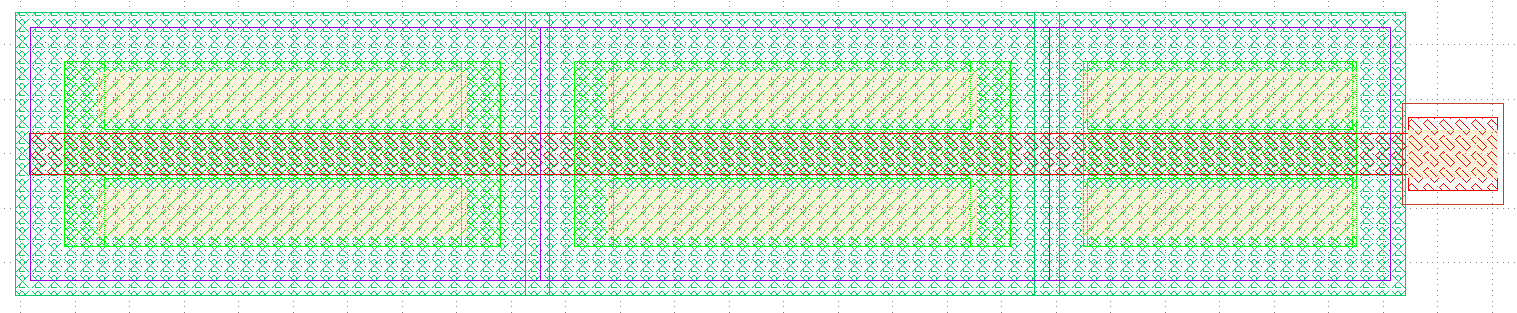
\includegraphics[width=0.25\textwidth]{figures/precharge_transistors.png}
\caption{The three base transistors of a precharge cell. \label{fig:precharge-transistors}}
\end{figure}

\begin{figure}[H] \centering
\begin{minted}{rust}
let params = LayoutMosParams {
  skip_sd_metal: vec![vec![]; 3],
  deep_nwell: true,
  contact_strategy: GateContactStrategy::SingleSide,
  devices: vec![
      MosParams {
          w: self.params.equalizer_width,
          l: self.params.length,
          m: 1,
          nf: 1,
          id: mos.id(),
      },
      MosParams {
          w: self.params.pull_up_width,
          l: self.params.length,
          m: 1,
          nf: 1,
          id: mos.id(),
      },
      MosParams {
          w: self.params.pull_up_width,
          l: self.params.length,
          m: 1,
          nf: 1,
          id: mos.id(),
      },
  ],
};

let mut mos = ctx.instantiate::<LayoutMos>(&params)?;
mos.set_orientation(Named::R90);
\end{minted}
\caption{A snippet of code for generating the precharge transistors shown in \ref{fig:precharge-transistors}. \label{fig:precharge-transistors-code}}
\end{figure}

Next, we allocate M1 routing tracks. At the left edge of the cell, the outermost half-tracks are used for routing VDD;
the inner two tracks are the bitlines. Towards the right side of the cell,
the bitline tracks move to make space for the gate contact.

These two routing regions are encoded using a \verb|FixedTracks| object in Substrate, connected by a \verb|SimpleJog|.
The \verb|FixedTracks| object produces tracks with a fixed line and space, centered in a given routing region.
It also accepts boundary conditions, which permit the user to place full tracks, half tracks, full spaces, or half spaces
at the edge of the routing region.

The \verb|SimpleJog| object allows the user to specify an arbitrary number of source tracks, and an equal number of destination tracks.
It then jogs each source track to the corresponding destination track.

A code snippet (lightly edited for clarity) and image of this stage of precharge cell generation are shown in \ref{fig:precharge-m1-routing-code} and \ref{fig:precharge-m1-routing}.

\begin{figure}[H] \centering
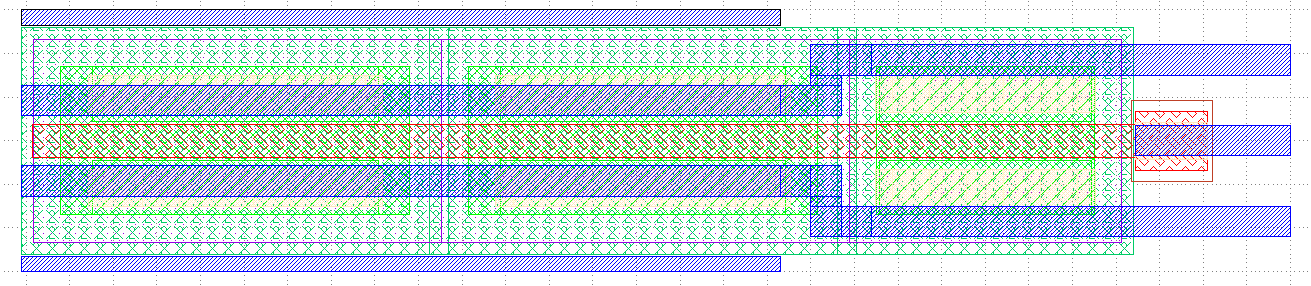
\includegraphics[width=0.75\textwidth]{figures/precharge_m1_routing.png}
\caption{Precharge cell metal 1 routing. \label{fig:precharge-m1-routing}}
\end{figure}

\begin{figure}[H] \centering
\begin{minted}{rust}
let in_tracks = FixedTracks::from_centered_tracks(CenteredTrackParams {
    line: 140,
    space: 230,
    span: Span::new(0, 1_200),
    num: 4,
    lower_boundary: Boundary::HalfTrack,
    upper_boundary: Boundary::HalfTrack,
    grid: 5,
});
let out_tracks = FixedTracks::from_centered_tracks(CenteredTrackParams {
    line: 140,
    space: 230,
    span: Span::new(0, 1_200),
    num: 3,
    lower_boundary: Boundary::HalfSpace,
    upper_boundary: Boundary::HalfSpace,
    grid: 5,
});

// ...

let mut orects = Vec::with_capacity(dsn.out_tracks.len());
for i in 0..dsn.out_tracks.len() {
    let top = if i == 1 { gate.top() } else { cut };
    let rect = Rect::from_spans(dsn.out_tracks.index(i), Span::new(0, top));
    ctx.draw_rect(dsn.v_metal, rect);
}

let jog = SimpleJog::builder()
    .dir(Dir::Vert)
    .src_pos(cut)
    .src([dsn.out_tracks.index(0), dsn.out_tracks.index(2)])
    .dst([dsn.in_tracks.index(1), dsn.in_tracks.index(2)])
    .line(dsn.v_line)
    .space(dsn.v_space)
    .layer(dsn.v_metal)
    .build()
    .unwrap();

for i in 0..dsn.in_tracks.len() {
    let rect = Rect::from_spans(
        dsn.in_tracks.index(i),
        Span::new(jog.dst_pos(), bbox.height()),
    );
    ctx.draw_rect(dsn.v_metal, rect);
}
\end{minted}
\caption{A snippet of code for generating precharge cell M1 routing.
The resulting layout is shown in \ref{fig:precharge-m1-routing}. \label{fig:precharge-m1-routing-code}}
\end{figure}


Next, we draw vias connecting the metal 1 tracks to transistor sources/drains/gates.
We also draw a power strap on metal 2 and drop vias to the VDD tracks on metal 1.
Sample code for drawing a via is shown in \ref{fig:sample-via-code}.
The \verb|ViaExpansion::LongerDirection| flag shown in that figure tells the via generator
that the via need not be contained in the overlap of the geometry on the top and bottom layers;
it can expand along the longer direction of the overlap region. This produces the 2x1 via arrays
seen in \ref{fig:precharge-vias}. If no expansion is permitted, Substrate fills the overlap region with as many
vias as possible. At least one via will be drawn, even if it does not fit entirely within the overlap region.

The precharge cell after drawing all vias and the power strap is shown in \ref{fig:precharge-vias}.

\begin{figure}[H] \centering
\begin{minted}{rust}
let mut via1 = ViaParams::builder()
  .layers(dsn.v_metal, dsn.h_metal)
  .expand(ViaExpansion::LongerDirection)
  .geometry(rects[0].double(Side::Left), stripe)
  .build();
let via = ctx.instantiate::<Via>(&via1)?;
ctx.draw(via)?;
\end{minted}
\caption{
Sample code snippet for drawing a via.
\label{fig:sample-via-code}
}
\end{figure}

\begin{figure}[H] \centering
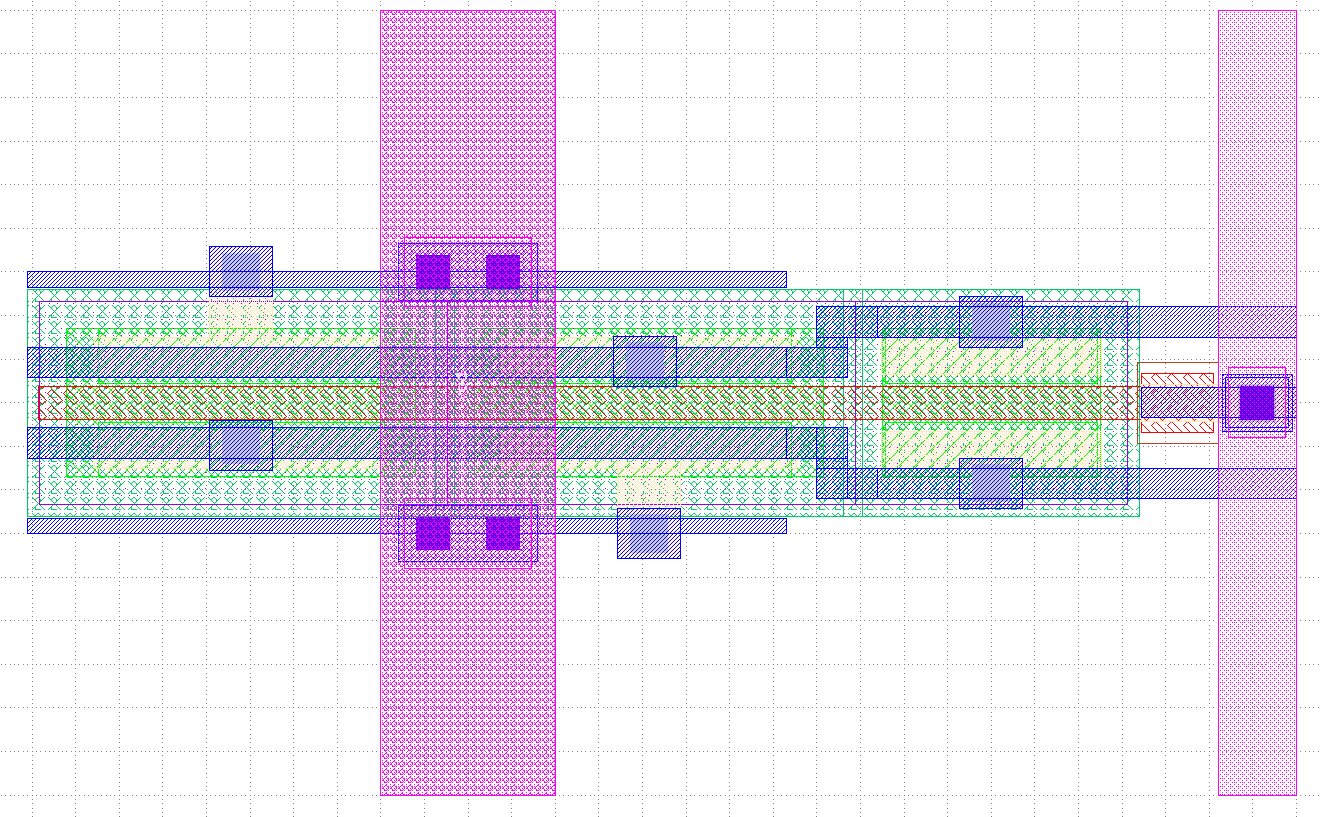
\includegraphics[width=0.75\textwidth]{figures/precharge_vias.png}
\caption{The precharge cell after drawing vias and a power strap. \label{fig:precharge-vias}}
\end{figure}


Finally, as shown in \ref{fig:precharge-trimmed}, we trim the precharge cell so that it can be tiled (using the tiling APIs described previously).

\begin{figure}[H] \centering
\begin{minted}{rust}
let bounds = ctx.brect().with_hspan(Span::new(0, dsn.width));
ctx.trim(&bounds);
\end{minted}
\caption{Trimming the precharge cell. \label{fig:precharge-trimmed}}
\end{figure}

There is an alternate convention for tiling cells, which is to skip the step of trimming the cell, and instead
allow adjacent cells to overlap. However, the convention of trimming cells is more convenient here for two reasons:
\begin{enumerate}
\item Substrate tilers place cells according to their bounding boxes. Tiling untrimmed cells would require wrapping them
  in a \verb|LayerBbox| tile (see \ref{sec:placement-utilities}) or manually specifying the bounding box to the tiler. Trimming the cell is more convenient than
  either of these options.
\item Special end cells are required to provide taps. So even if we were to tile untrimmed cells, we would still need to specify custom cells for
  the array edges and tap columns.
\end{enumerate}

The precharge cells illustrate how Substrate APIs can be used to produce very compact layout.
Much of the SRAM peripheral circuitry is generated in a similar manner. An image of the peripheral circuitry layout
is shown in \ref{fig:peripheral-circuitry-layout}. We omit specific discussion of the generators for the rest of the column
components, since they are similar in principle to the precharge cell.

\begin{figure}[H] \centering
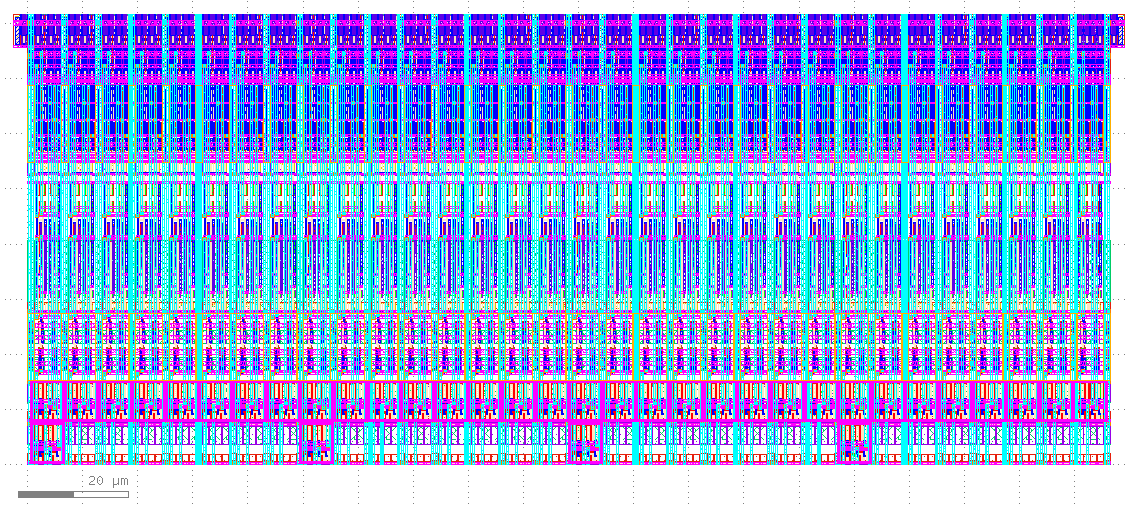
\includegraphics[width=\textwidth]{figures/col_peripherals.png}
\caption{Tiled column peripheral circuitry. The precharge cells occupy the topmost row. \label{fig:peripheral-circuitry-layout}}
\end{figure}

\subsection{Control Logic} \label{sec:control-logic-layout}

The control logic is a small $\left( \approx 100\right)$ set of logic gates that control the sequence of events during read and write operations.

Despite being entirely digital, using a traditional digital flow to lay out the control logic is undesirable:
\begin{itemize}
\item The control logic is pulsed, unlike the typical digital circuits for which these tools are optimized.
\item Minimizing area is important.
\item SRAM22 tries not to depend on commercial tools, and open source digital tool flows are not very mature.
\item Dependency on external tools would make SRAM22 more difficult and less convenient to use.
\end{itemize}

Therefore, we opt instead to place and route the control logic entirely within SRAM22 and Substrate.

The flow for using digital standard cells in Substrate is:
\begin{enumerate}
\item Import the desired standard cell libraries into Substrate.
\item Place the standard cells, often using a \verb|GridTiler| (\ref{sec:placement-utilities}) with tiles taking their bounding box from a ``PR boundary'' layer.
\item Select routing layers and define a routing grid for each layer.
\item Route between the placed standard cells.
\end{enumerate}

The fourth step is often done with a combination of manual routing and automatic routing.
SRAM22 uses manual routing when drawing routes than run solely on the local interconnect layer in SKY130.
For longer distance routes that span other metal layers, SRAM22 defers routing to the automatic router in Substrate.

We will focus on the use of the automatic router in this section, since this feature is, as far as we are aware, not present
in other analog generator frameworks. The router implementation in Substrate is called \verb|GreedyRouter|, as it creates
routes as they are specified, rather than trying to find a globally optimal routing solution.

To initialize the router, we specify a routing region and a set of routing layers. Each routing layer holds the
line and space of tracks on that layer, a preferred routing direction, and a reference to a PDK layer.
Router intialization is shown in \ref{fig:greedy-router-initialization}.

\begin{figure}[H] \centering
\begin{minted}{rust}
let mut router = GreedyRouter::with_config(GreedyRouterConfig {
    area: group.brect().expand(1840),
    layers: vec![
        LayerConfig {
            line: 320,
            space: 140,
            dir: Dir::Horiz,
            layer: m1,
        },
        LayerConfig {
            line: 320,
            space: 140,
            dir: Dir::Vert,
            layer: m2,
        },
    ],
});
\end{minted}
\caption{Greedy router initialization with two metal layers (M1 and M2). \label{fig:precharge-m1-routing-code}}
\end{figure}

The current implementation of \verb|GreedyRouter| only permits on-grid routing.
However, cells being routed may have off-grid pins. These pins must be jogged onto
the routing grid before asking the router to route from/to them. Substrate
provides an \verb|expand_to_grid| function for doing this. An example usage is shown in \ref{fig:router-expand-to-grid}.
Users specify a rectangle representing the off-grid pin and an expansion strategy. The router
will automatically find an appropriate on-grid point to which the off-grid pin can be connected,
consistent with the expansion strategy. Possible expansion strategies include:
\begin{itemize}
\item Minimum area: connect to the routing grid using the minimum amount of extra metal area.
\item Top/bottom/left/right: connect to the nearest grid point to the given side of the source pin.
\item Upper left/lower left/upper right/lower right: connect to the nearest grid point off of the given corner of the source pin.
\end{itemize}

\begin{figure}[H] \centering
\begin{minted}{rust}
let clkp_out = router.expand_to_grid(
    clkp_out_via.layer_bbox(m1).into_rect(),
    ExpandToGridStrategy::Minimum,
);
router.occupy(m1, clkp_out, "clkp")?;
\end{minted}
\caption{Expanding the (pulse generator output) pin to the routing grid. \label{fig:precharge-m1-routing-code}}
\end{figure}


Substrate also has more sophisticated routines for bringing off-grid geometry onto the routing grid.
For example, users can ask the Substrate router to jog a bus of off-grid pins onto adjacent routing tracks.
The router will calculate the minimum necessary amount of spacing in the routing layer's preferred routing direction.
The router logic can handle a wide range of off-grid pitches, and can handle cases where the off-grid bus is not centered
with the target on-grid tracks. An example of the geometry generated by this procedure is shown in \ref{fig:off-grid-routing}.

\begin{figure}[H] \centering
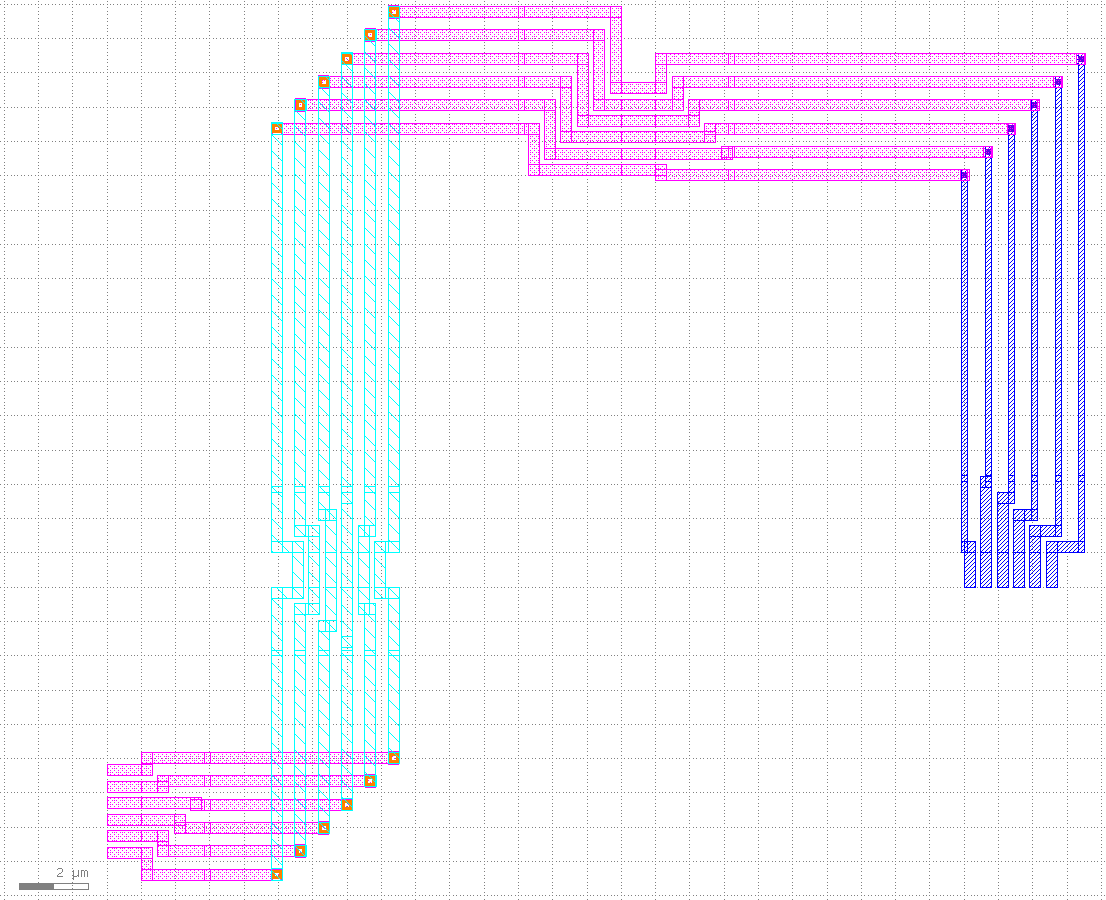
\includegraphics[width=\textwidth]{figures/off_grid_routing.png}
\caption{A sample of the geometry automatically generated by the router to bring off-grid pins to the routing grid. \label{fig:off-grid-routing}}
\end{figure}


Bringing off-grid pins to the routing grid is by far the most tedious part of generating layouts based on
digital standard cells. Further improvements to Substrate have the potential to make this process easier.

Once all geometry is on-grid, routing becomes very easy (see \ref{fig:auto-routing}).

\begin{figure}[H] \centering
\begin{minted}{rust}
router.route_with_net(ctx, m1, clkp_out, m1, clkp_in_1, "clkp")?;
router.route_with_net(ctx, m1, clkp_out, m1, clkp_in_2, "clkp")?;
router.route_with_net(ctx, m1, clkp_out, m1, clkp_in_3, "clkp")?;
\end{minted}
\caption{Routing the clock pulse generator output to three consumers. \label{fig:auto-routing}}
\end{figure}
    % Routing the clock pulse generator output \texttt{(\verb|clkp_out|)} to three consumers \texttt{(\verb|clkp_in_1|, \verb|clkp_in_2|, \verb|clkp_in_3|)}.
    % The net name "clkp" identifies that each route is on a net called "clkp"; this tells the router that it can
    % reuse any geometry previously drawn on the same net. Without this, a naive routing implementation might try to find
    % separate, independent routes from \texttt{\verb|clkp_out|} to each of the three targets.

By issuing several of these routing commands, the full layout can be programatically routed. Extracting these
routing paths from a schematic view is possible in principle, but has not been implemented at the time of writing.

The fully-routed layout of SRAM22's control logic is shown in \ref{fig:control-logic-routed-layout}. The output pins are placed towards
the upper right for convenience in top-level routing.

\begin{figure}[H] \centering
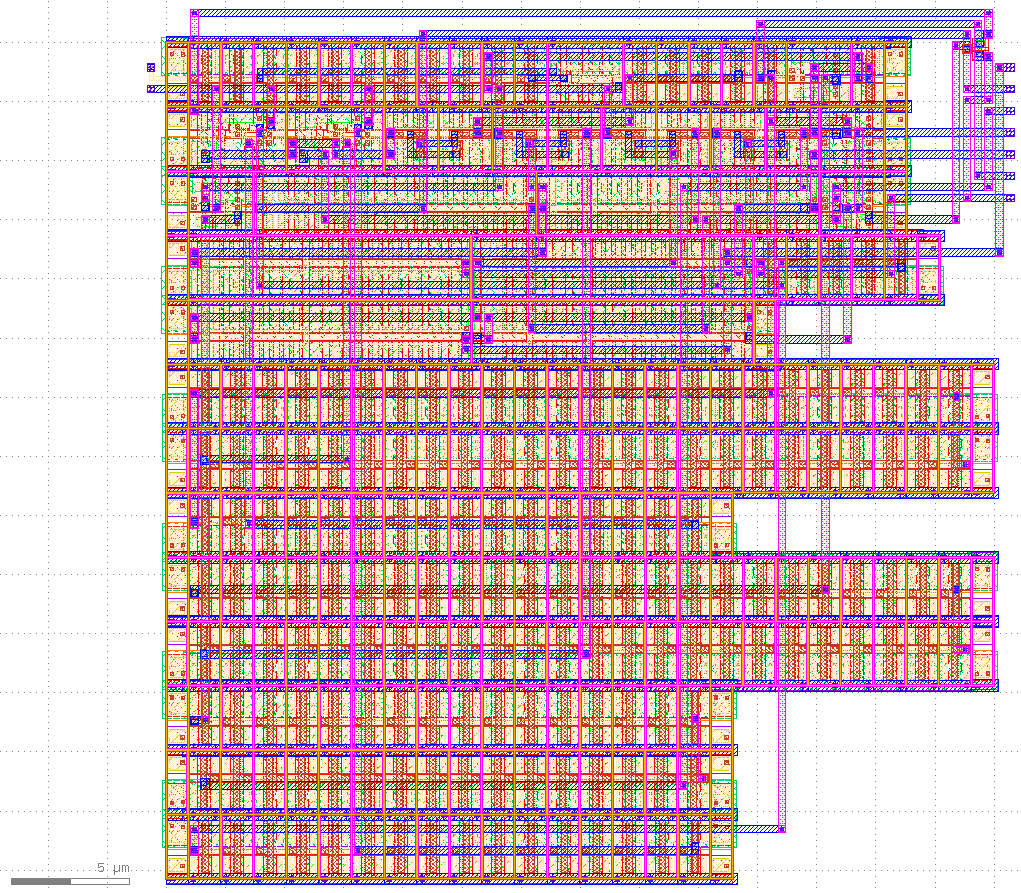
\includegraphics[width=\textwidth]{figures/control_logic_layout.png}
\caption{The control logic cell in SRAM22. Most routing is done via the automatic router in Substrate. \label{fig:control-logic-routed-layout}}
\end{figure}

